%%%%%%%%%%%%%%%%%%%%%%%%%%%%%%%%%%%%%%%%%%%%%%%%%%%%%%%%%%%%%%%%%%%%%%
%%                     Not
%%%%%%%%%%%%%%%%%%%%%%%%%%%%%%%%%%%%%%%%%%%%%%%%%%%%%%%%%%%%%%%%%%%%%%
%\color{blue}
\subsubsection{Glyph: \glyph{Not}}\label{sec:not}

The glyph \glyph{not} is used to denote that the output influence only happens in the absence of the input \glyph{entity node}.

\begin{glyphDescription}

 \glyphSboTerm SBO:0000238 ! not.

 \glyphContainer \glyph{Not} is represented by a circle, with two connectors located at the opposite side for input and output.

  \glyphLabel \glyph{Not} is identified by the label ``NOT'' placed in an unbordered box attached to the center of the container. 

  \glyphAux \glyph{Not} does not carry any auxiliary items.

\end{glyphDescription}

\begin{figure}[H]
  \centering
  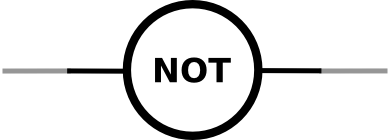
\includegraphics[scale = 0.5]{images/not}
  \caption{The \ER glyph for \glyph{not}.}
  \label{fig:not}
\end{figure}

